\newif\ifshowsolutions
\showsolutionstrue
\documentclass{article}
\usepackage{listings}
\usepackage{amsmath}
%\usepackage{subfigure}
\usepackage{subfig}
\usepackage{amsthm}
\usepackage{amsmath}
\usepackage{amssymb}
\usepackage{graphicx}
\usepackage{mdwlist}
\usepackage[colorlinks=true]{hyperref}
\usepackage{geometry}
\usepackage{titlesec}
\geometry{margin=1in}
\geometry{headheight=2in}
\geometry{top=2in}
\usepackage{palatino}
\usepackage{mathrsfs}
\usepackage{fancyhdr}
\usepackage{paralist}
\usepackage{todonotes}
\setlength{\marginparwidth}{2.15cm}
\usepackage{tikz}
\usetikzlibrary{positioning,shapes,backgrounds}
\usepackage{float} % Place figures where you ACTUALLY want it
\usepackage{comment} % a hack to toggle sections
\usepackage{ifthen}
\usepackage{mdframed}
\usepackage{verbatim}
\usepackage[strings]{underscore}
\usepackage{listings}
\usepackage{bbm}
\rhead{}
\lhead{}

\renewcommand{\baselinestretch}{1.15}

% Shortcuts for commonly used operators
\newcommand{\E}{\mathbb{E}}
\newcommand{\Var}{\operatorname{Var}}
\newcommand{\Cov}{\operatorname{Cov}}
\newcommand{\Bias}{\operatorname{Bias}}
\DeclareMathOperator{\argmin}{arg\,min}
\DeclareMathOperator{\argmax}{arg\,max}

% do not number subsection and below
\setcounter{secnumdepth}{1}

% custom format subsection
\titleformat*{\subsection}{\large\bfseries}

% set up the \question shortcut
\newcounter{question}[section]
\newenvironment{question}[1][]
  {\refstepcounter{question}\par\addvspace{1em}\textbf{Question~\Alph{question}\!
    \ifthenelse{\equal{#1}{}}{}{ [#1 points]}: }}
    {\par\vspace{\baselineskip}}

\newcounter{subquestion}[question]
\newenvironment{subquestion}[1][]
  {\refstepcounter{subquestion}\par\medskip\textbf{\roman{subquestion}.\!
    \ifthenelse{\equal{#1}{}}{}{ [#1 points]:}} }
  {\par\addvspace{\baselineskip}}

\titlespacing\section{0pt}{12pt plus 2pt minus 2pt}{0pt plus 2pt minus 2pt}
\titlespacing\subsection{0pt}{12pt plus 4pt minus 2pt}{0pt plus 2pt minus 2pt}
\titlespacing\subsubsection{0pt}{12pt plus 4pt minus 2pt}{0pt plus 2pt minus 2pt}


\newenvironment{hint}[1][]
  {\begin{em}\textbf{Hint: }}{\end{em}}

\ifshowsolutions
  \newenvironment{solution}[1][]
    {\par\medskip \begin{mdframed}\textbf{Solution~\Alph{question}#1:} \begin{em}}
    {\end{em}\medskip\end{mdframed}\medskip}
  \newenvironment{subsolution}[1][]
    {\par\medskip \begin{mdframed}\textbf{Solution~\Alph{question}#1.\roman{subquestion}:} \begin{em}}
    {\end{em}\medskip\end{mdframed}\medskip}
\else
  \excludecomment{solution}
  \excludecomment{subsolution}
\fi

\newcommand{\boldline}[1]{\underline{\textbf{#1}}}

\chead{%
  {\vbox{%
      \vspace{2mm}
      \large
      Machine Learning \& Data Mining \hfill
      Caltech CS/CNS/EE 155 \hfill \\[1pt]
      Miniproject 1\hfill
      Released January $29^{th}$, 2018 \\
    }
  }
}

\begin{document}
\pagestyle{fancy}



\section{Introduction}
\medskip
\begin{itemize}

    \item \boldline{Group members} \\
    Aw Young Qingzhuo, Ola Kalisz, and Riley Patterson
    
    \item \boldline{Team name} \\
    Not Hotdog
    
    \item \boldline{Division of labour} \\
    TODO: document this after project is done

\end{itemize}



\section{Overview}
\medskip
\begin{itemize}

    \item \boldline{Models and techniques tried}

        Our overall approach was to stack the results of a wide variety of ``first layer'' models to train a ``second layer'' ensemble model.
        % TODO describe the stacking approach in a bit more detail in this section, either here or after the lists of models.

        For \textbf{first layer models}, we experimented with each of the following, only a subset of which we ended up using in our final model.
        \begin{itemize}
            \item \textbf{K Nearest Neighbors:} Trained KNN for a wide range of $N \in \{2^i | i \in [1,10]\}$ with three different distance metrics for each $N$: Manhattan, Euclidean, and Bray-Curtis.
            \item \textbf{AdaBoost:} with hyperparameter selection across the number of estimators and the learning rate.
            \item \textbf{Random Forest:} with hyperparameter selection across the max depth and minimum split size, with number of estimators set at 250.
            \item \textbf{Extra Trees:} % TODO blurb
            \item \textbf{XGBoost:} % TODO blurb
            \item \textbf{Logistic Regression:} % TODO blurb
            \item \textbf{FFM:} % TODO blurb
            \item \textbf{Vowpal-Wabbit:} % TODO blurb
            \item \textbf{Neural Nets:} to incorporate data from other representations including:
                \begin{itemize}
                    \item Embeddings % TODO blurb, did we actually use this in practice? can't tell from the colab or the notebook
                    % TODO more info on neural nets
                \end{itemize}
        \end{itemize}

        For \textbf{second layer models}, we experimented with each of the following:
        \begin{itemize}
            \item \textbf{Neural Net:} constructed with two dense hidden layers whose sizes we experimented with, and a number of dropout layers for regularization.
            \item \textbf{Logistic Regression:} % TODO(riley) blurb
        \end{itemize}

    \item \boldline{Work timeline}
    \begin{itemize}
    % Insert text here. Bullet points can be made using '\item'.
    \item \textbf{Bullet:} Bullet text.
    \end{itemize}

\end{itemize}



\section{Approach}
\medskip
\begin{itemize}

    \item \boldline{Data processing and manipulation}
    \begin{itemize}
    % Insert text here. Bullet points can be made using '\item'.
        \item \textbf{Bag of Words:} Most models relied on the bag-of-words representation provided with no modification before input to our first layer models
        % TODO(qingzhuo): some thoughts on attempts to reverse the stemming process and use word2vec/other representations
        \item \textbf{Second Layer Model Meta-Features:} % TODO decide whether to talk about this here or somewhere else, e.g. in second level details in the next section
    \end{itemize}

    \item \boldline{Details of models and techniques}

        % NB: perhaps we should actually put the results of parameter search in the Model Selection->Scoring section?
        We optimized \textbf{first layer models} in isolation, with results detailed below:
        \begin{itemize}
            \item \textbf{K Nearest Neighbors:} Trained KNN for a wide range of $N \in \{2^i | i \in [1,10]\}$ with three different distance metrics for each $N$: Manhattan, Euclidean, and Bray-Curtis.
                % TODO(riley) KNN performance based on inference data
            \item \textbf{AdaBoost:} with hyperparameter selection across the number of estimators and the learning rate.
                % TODO(ola) data from wiki
                \begin{figure}[H]
                \centering
                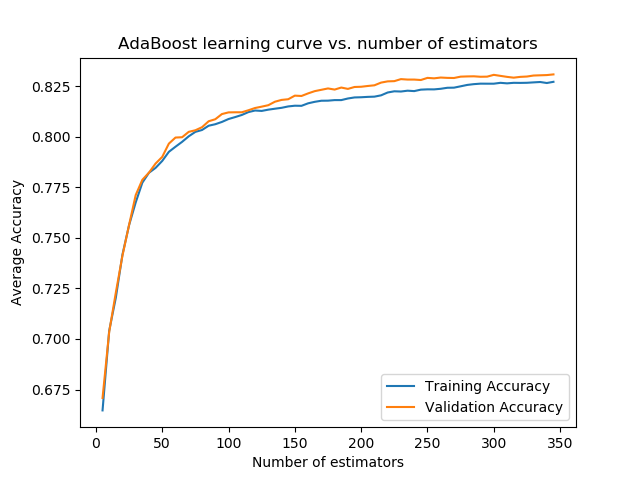
\includegraphics[width=\textwidth]{adaboost_vs_nest.png}
                \caption{AdaBoost training and validation accuracy vs. number of estimators.}
                \end{figure}
            \item \textbf{Random Forest:} with hyperparameter selection across the max depth and minimum split size, with number of estimators set at 250.
                % TODO(ola) data from wiki
                % TODO(riley) graph
            \item \textbf{Extra Trees:} % TODO details
            \item \textbf{XGBoost:} % TODO details
            \item \textbf{Logistic Regression:} % TODO details
            \item \textbf{FFM:} % TODO details
            \item \textbf{Vowpal-Wabbit:} % TODO details
            \item \textbf{Neural Nets:} to incorporate data from other representations including:
                \begin{itemize}
                    \item Embeddings % TODO details
                    % TODO more info on neural nets
                \end{itemize}
        \end{itemize}

        For \textbf{second layer models}, we found:
        \begin{itemize}
            \item \textbf{Neural Net:}
                % TODO(riley) comments on overfitting
            \item \textbf{Logistic Regression:}
                % TODO(riley) comments on overfitting both before/after model candidate reduction
        \end{itemize}

\end{itemize}



\section{Model Selection}
\medskip
\begin{itemize}

    \item \boldline{Scoring} \\
        % TODO are we supposed to write about the accuracy metric used in this section, and how we interpreted it?
        % TODO(riley) likely write about attempt to prevent data leaking into the second layer here, how that didn't work and how we would fix it in the future

    \item \boldline{Validation and Test} \\
        % TODO(riley) comments/figure on final model selection vs. all models in second layer
        % TODO possibly create a table showing all model validation/test scores
    % Insert text here.

\end{itemize}



\section{Conclusion}
\medskip
\begin{itemize}

    \item \boldline{Discoveries} \\
    % Insert text here.

    \item \boldline{Challenges} \\
    % Insert text here.

    \item \boldline{Concluding Remarks} \\
    % Insert text here.

\end{itemize}



\end{document}
